%------------------------------------------------------------------------
%Editar Diplomado
\hypertarget{cv:eliminarMensaje}{\section{Eliminar Mensaje}} \label{sec:eliminarMensaje}

	Esta funcionalidad le permitirá eliminar un mensaje innecesario o incorrecto. Para eliminar un mensaje es necesario que no se encuentre asociado a casos de uso.

		\subsection{Procedimiento}

			%Pasos de procedimiento
			\begin{enumerate}
	
			\item Oprima el botón \IUBotonEliminar{} de un registro existente de la pantalla \ref{fig:GestionarMensajes} ''Gestionar Mensajes''.
	
			\item Se mostrará el mensaje \ref{fig:confirmaEliminaMensaje} sobre la pantalla \ref{fig:GestionarMensajes} ''Gestionar Mensajes''.
			
			%Pantalla
			\begin{figure}[htbp!]
				\begin{center}
					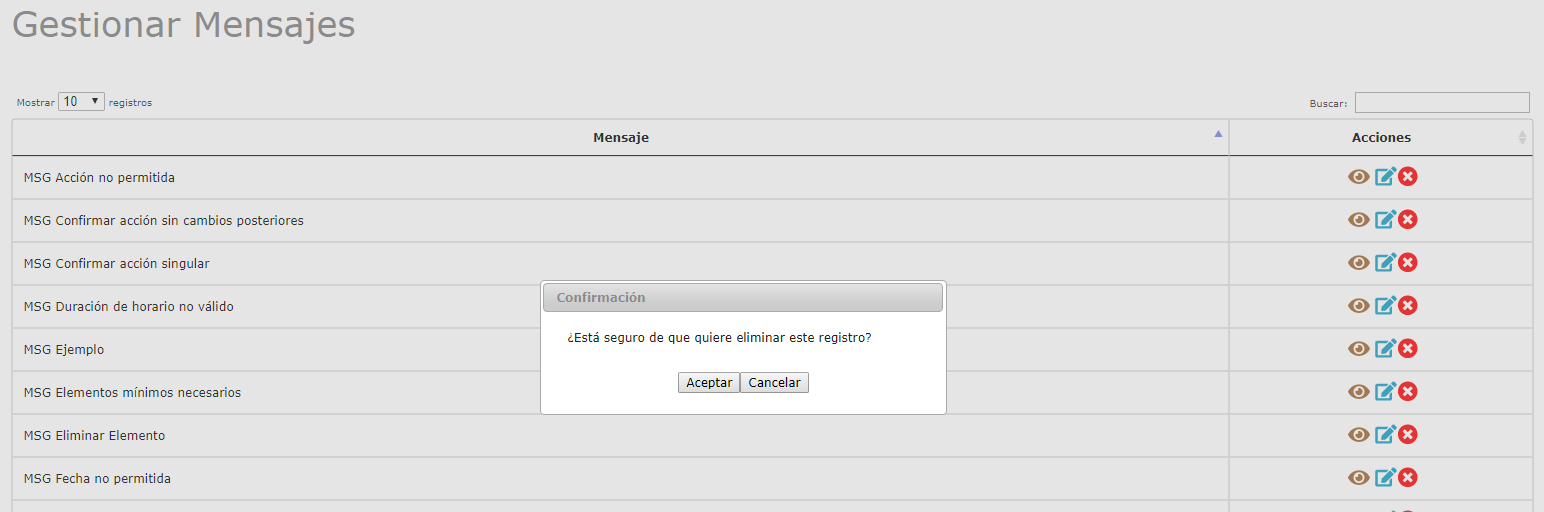
\includegraphics[scale=0.40]{roles/lider/mensajes/pantallas/IU9-3MSG10}
					\caption{MSG de Confirmación}
					\label{fig:confirmaEliminaMensaje}
				\end{center}
			\end{figure}
						
			\item Oprima el botón \IUAceptar.
			
			\item Se mostrará el mensaje \ref{fig:mensajeEliminado} en la pantalla \ref{fig:GestionarMensajes} ''Gestionar Mensajes''.
			
			\begin{figure}[htbp!]
				\begin{center}
					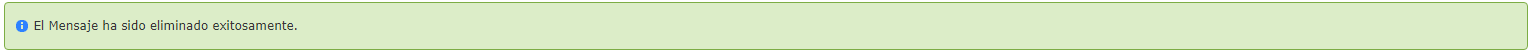
\includegraphics[scale=0.40]{roles/lider/mensajes/pantallas/IU9-3MSG1}
					\caption{MSG: Mensaje Eliminado}
					\label{fig:mensajeEliminado}
				\end{center}
			\end{figure}
			\end{enumerate}